\section{System Overview}

Pixels is an adaptive storage system on top of HDFS.
As shown in Figure~\ref{fig:overview}, it contains four functional modules:
\begin{itemize}
	\item \textit{Streaming Data Ingestion}. Unlike traditional ETL process on HDFS in which data is transformed into specific format in a batch manner, in Pixels, data is ingested into the system in streaming manner. We assume that the analytical workload mostly accesses the most recent data, so that we do not reload the historical data. When the Layout optimizer generates a new data layout, it is only applied on the new coming data.
	
	\item \textit{Workload Modeling}. Workload modeling is responsible for collecting the query workload and build workload models. Access patterns (columns accessed by queries) and filters (predicates) of the queries are collected by this module.
	Then the access patterns and filters are used to build a workload model by which we can predict the access patterns and filters in the coming future. In pixels, we use hidden Markov chain the model the workload.
	
	\item \textit{Reading Optimizer}. Read optimizer is a query optimizer embedded in Pixels, i.e. the storage layer in a data analytic system. Different from the traditional query optimizer in database systems, reading optimizer is only responsible for optimizing the data accessing behaviors in the storage layer, such as how many row groups are read by a data reading (map) task.
	Besides optimizing data reading tasks, reading optimizer also collects and maintains the data reading costs, which are used to build the data reading cost model. Data statistics are also collected and maintained by \textit{Reading Optimizer}. Such statistics are used by \textit{Reading Optimizer} to optimize the reading tasks and used by \textit{Streaming Data Ingestion} module to optimize data encoding and indexing.
	
	\item \textit{Layout Optimizer}. Layout optimizer optimizes the data layout with the workload model built by \textit{Workload Modeling} module and the reading cost model built by \textit{Reading Optimizer}. Data layout optimization is triggered by workload modeling module when the workload model is significantly changed. The new data layout generated and evaluated by layout optimizer is then provided to \textit{Streaming Data Ingestion} module to be applied in the new coming data.
	
	
\end{itemize}


\begin{figure}[h!]
	\vspace{-1em}
	\centering
	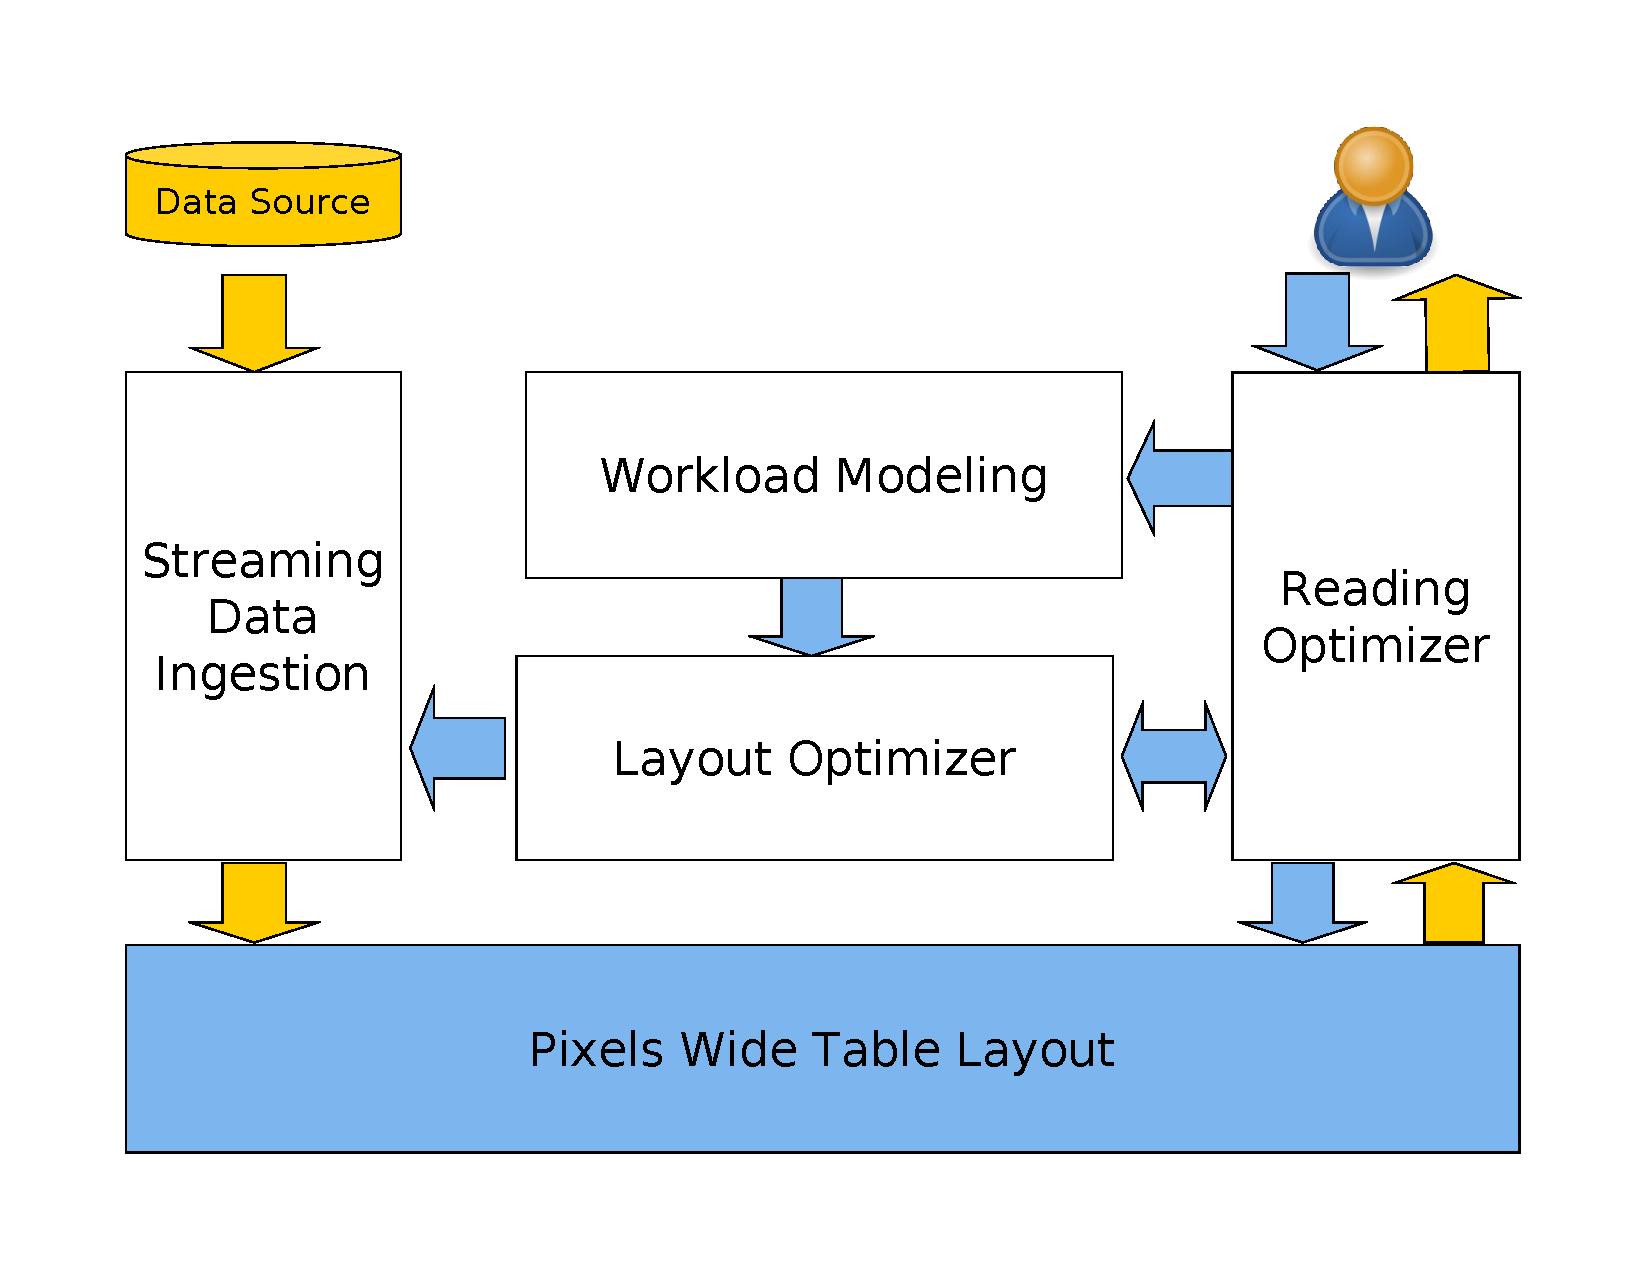
\includegraphics[width=0.5\textwidth, height=0.36\textwidth]{figs/overview}
	\vspace{-3em}
	\caption{System modules in Pixels}\label{fig:overview}
	\vspace{-0em}
\end{figure}

\subsection{Workload Modeling}
\label{subsec:workload-modeling}


\subsection{Optimizer in the Loop}
\label{subsec:optimizer-in-the-loop}

\begin{figure}[h!]
	\vspace{-3em}
	\centering
	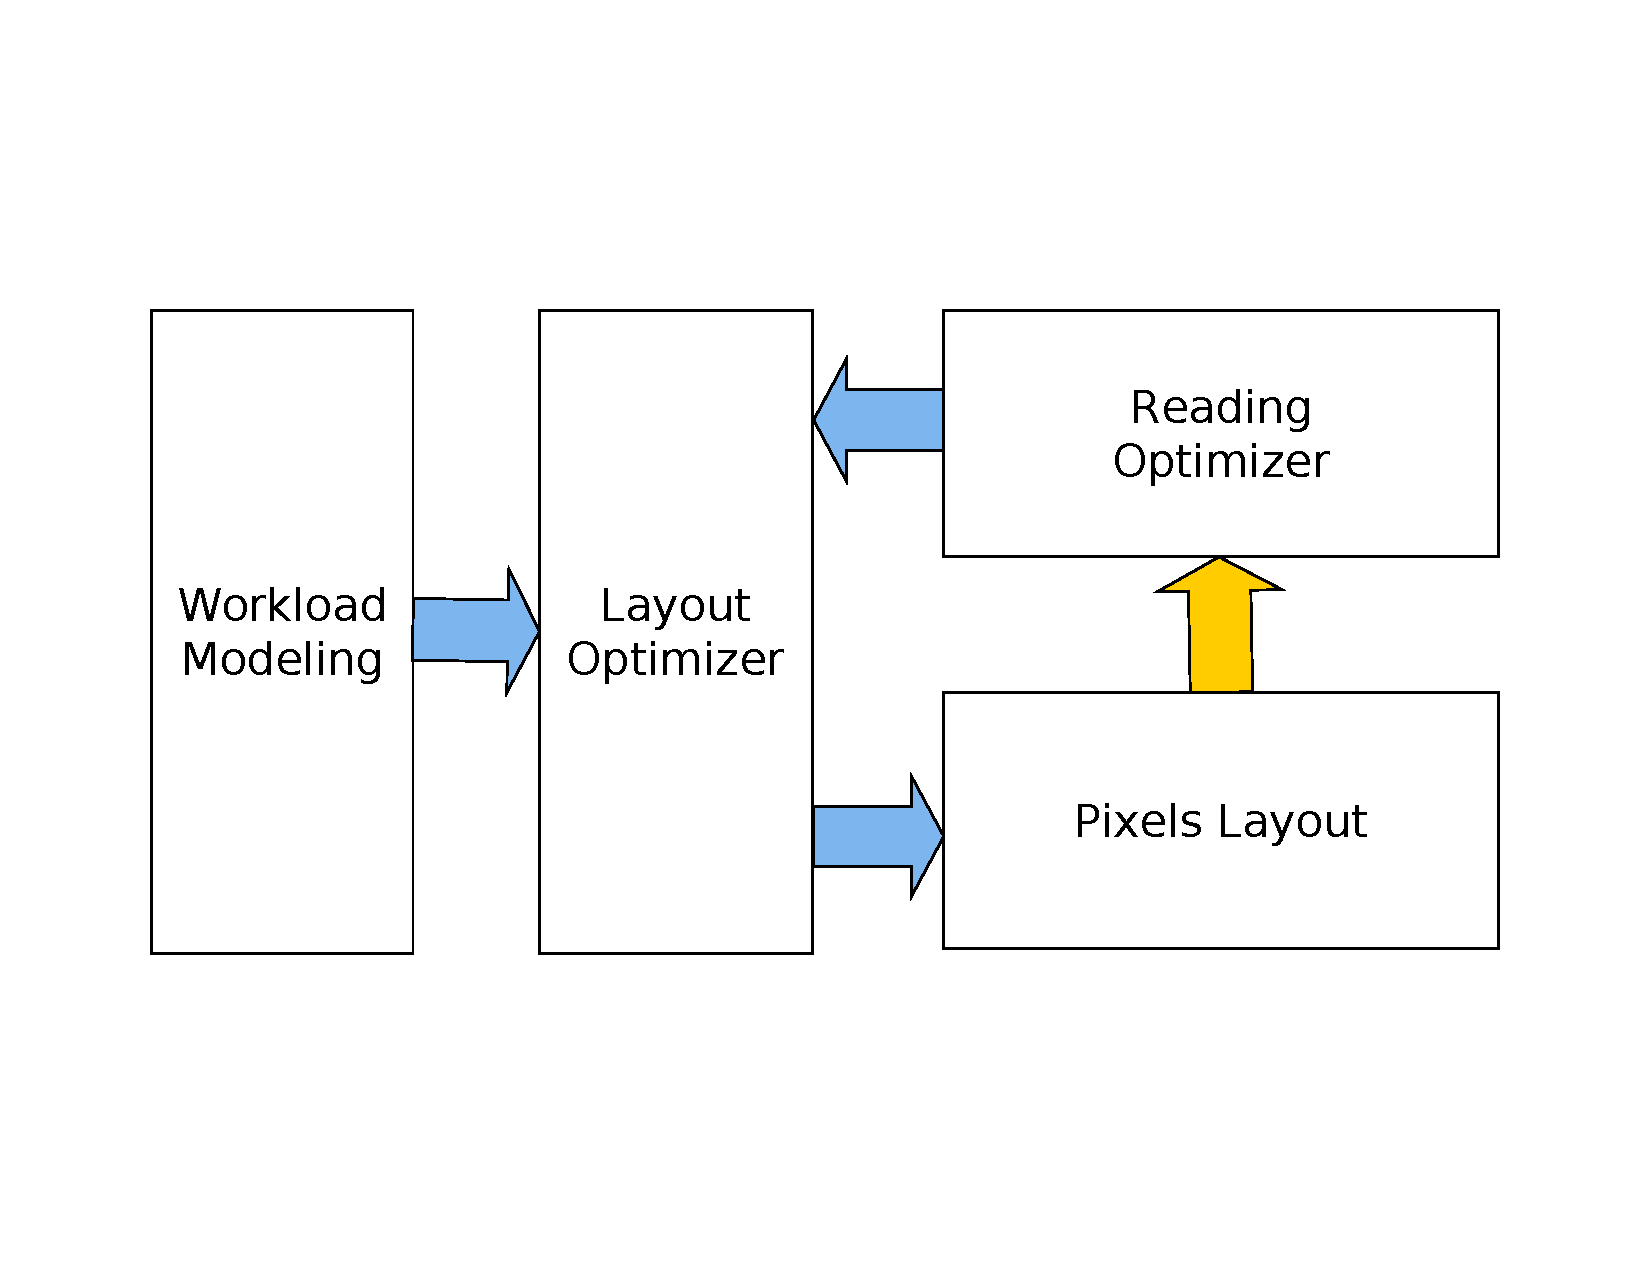
\includegraphics[width=0.5\textwidth, height=0.36\textwidth]{figs/loop}
	\vspace{-6em}
	\caption{Optimizer in the Loop}\label{fig:loop}
	\vspace{-0em}
\end{figure}


\section{Column Chunk Ordering}
\label{subsec:column-chunk-ordering}
